\documentclass{article}

\usepackage{graphicx, float, blindtext} % for dummy text
\usepackage{amsmath}
\graphicspath{ {./images/} }
\title{Chapter 10: Model comparison and Hierachical Modelling}
\author{Shubham Gupta}

\begin{document}
\maketitle
\section{Introduction}
\begin{itemize}
    \item When we have multiple models describing the same data, we need to assign credibilities to each model.
    \item Bayesian model comparison reallocates credibility across models given the data.  
    \item Model comparison $\implies$ bayesian estimatation of hierachical models where the top-level is the index of the models.
\end{itemize}
\section{Bayes Factor}
\subsection{General Formula}
\begin{itemize}
    \item Assume we have data $D$ with parameters $\theta$.
    \item Prior distribution is $p(\theta)$
    \item Parameter  $m$ to specify the index of the model.
    \item Hence, we will get
        \[
            likelihood = p_{m}(y|\theta_{m}, m)
        .\] 
        \[
            prior = p(\theta_{m}|m) 
        .\]                 

    \item Priors have different subscripts because they might have different distributions for each model.
    \item Assume each model is given a prior probability of $p(\theta)$. Then, for all possible models $\theta_{1}, \theta_{2}\ldots m$, we have:
        \[
            p(\theta_{1}, \theta_{2} \ldots | D) = \frac{P(D | \theta_{1}, \theta_{2} \ldots m) * p(\theta_{1}, \theta_{2} \ldots m)}{\sum_{m} \int d\theta_{m}p(D| \theta_{1}, \theta_{2} \ldots m) p(\theta_{1}, \theta_{2} \ldots m)} 
        .\] 
        \begin{figure}[H]
            \centering
            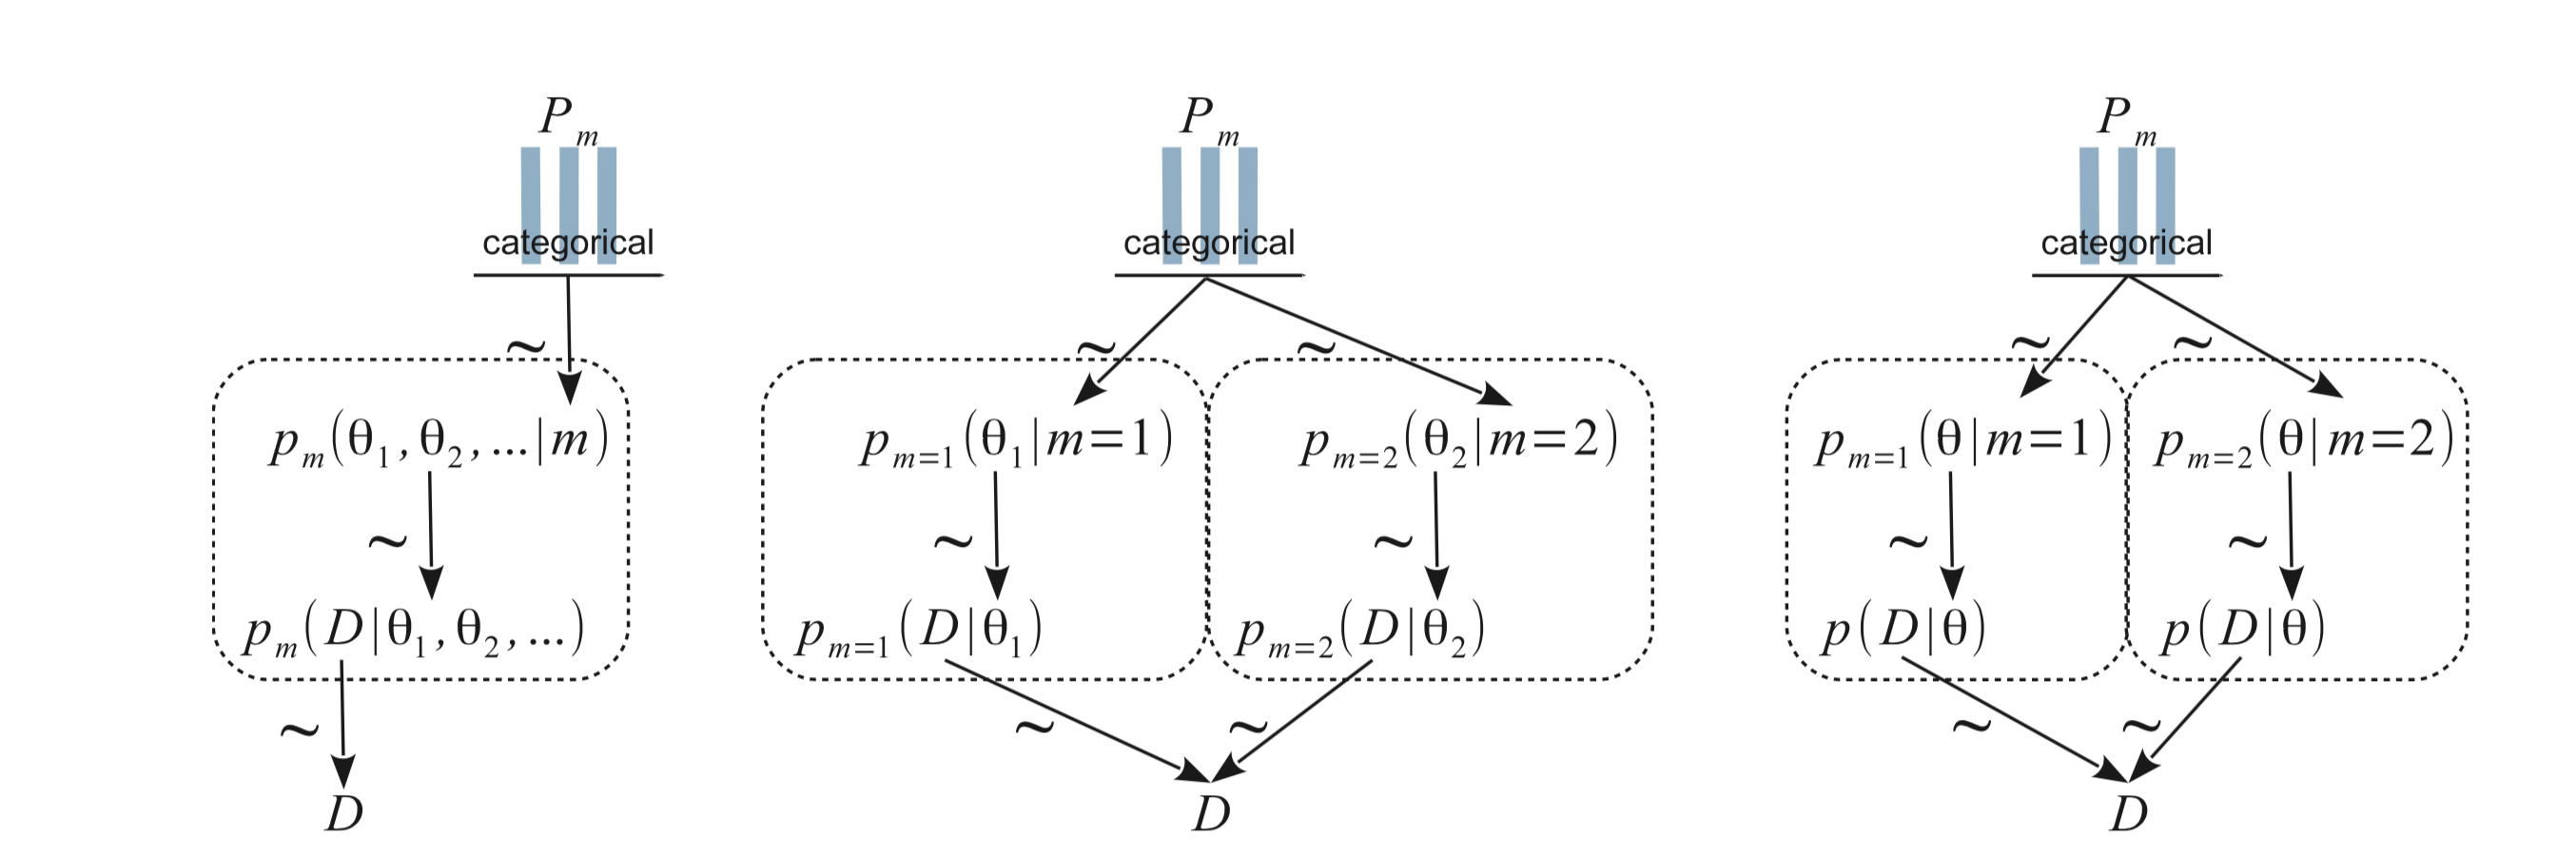
\includegraphics[width=0.8\textwidth]{model_index}
            \caption{Model comparisons as a hierachical model}
            \label{fig:model_index}
        \end{figure} 
    \item To get the relative probabilities of the models, we will divide their posterior outputs.
        \[
            \frac{p(m=1 | D)}{p(m=2 | D)} = \frac{p(D | m = 1) * p(m=1) / \sum_{m}P(D|m) * p(m)}{p(D | m = 2) * p(m=2) /\sum_{m}P(D|m) * p(m)}
        .\] 
    \item The above equation is called the Bayes Factor
    \item We can use the below table for reference on figuring out when to report a model is better than the alternative model.
        \begin{figure}[H]
            \centering
            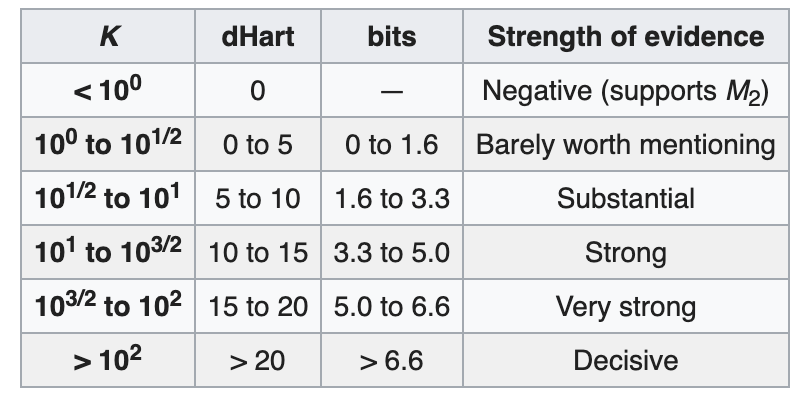
\includegraphics[width=0.8\textwidth]{bayes_factor}
            \caption{bayes factor}
            \label{fig:bayes_factor}
        \end{figure} 
\end{itemize}
\section{Head biased vs tail biased factories}
\begin{itemize}
    \item Two factories that produce head-biased and tail biased factories. Given we have seen some tosses, which factory did the coin come from?
    \item We have the following hierachy
        \begin{figure}[H]
            \centering
            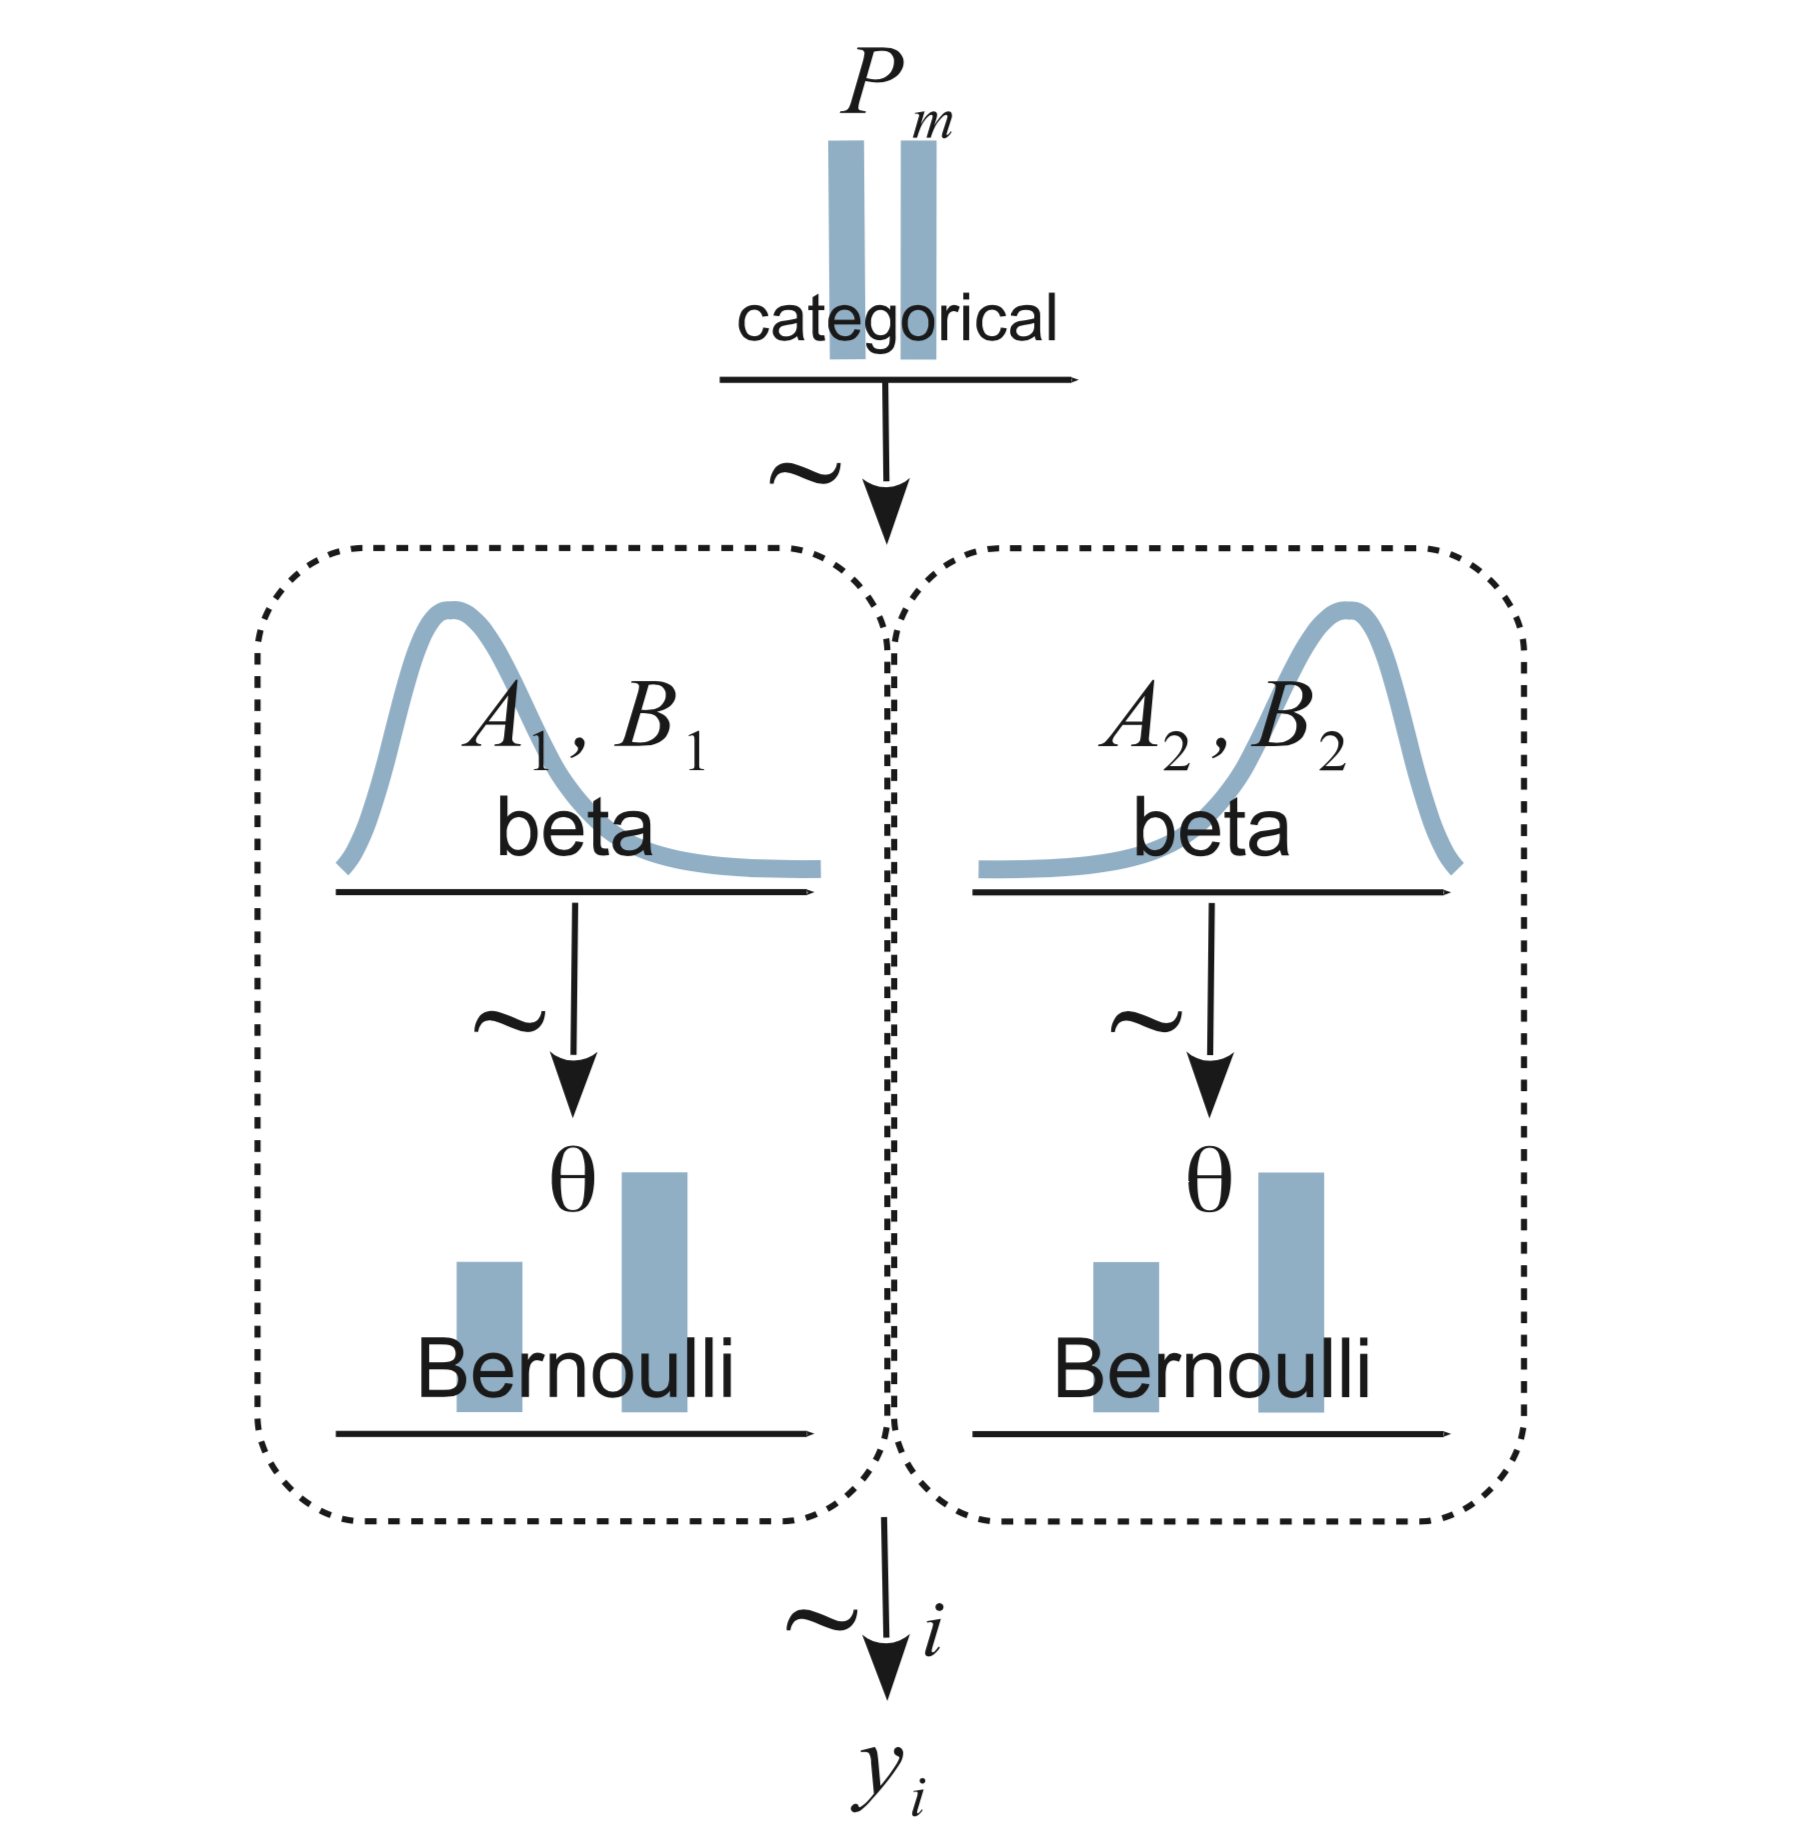
\includegraphics[width=0.8\textwidth]{coin_model_hierachy}
            \caption{Coin Model Hierachy}
            \label{fig:coin_model_hierachy}
        \end{figure}
\end{itemize}
\subsection{MCMC Method: Individual models}
\begin{itemize}
    \item Main formula to compute the probability of the data is:
    \[
        \frac{1}{p(D)} = \frac{1}{N} \sum_{n=\theta_{i} \tilde p(\theta|D)}^{N} \frac{h(\theta_{i})}{p(D|\theta_{i}) p(\theta_{i})} 
    .\]     
\item $h(\theta_{i}$ is a probability density function. There is a complex derivation to this formula, which we are skipping for now. Refer to page 275.
\end{itemize}
\subsection{MCMC Method: Hierachical model}
\begin{itemize}
    \item Similar to pymc3 models you have used. Use a index `m` to indicate for which model are the parameters being specified.
    \item 
\end{itemize}

\end{document}
